% Nejprve uvedeme tridu dokumentu s volbami
\documentclass[czech,public,dept460,male,cpdeclaration]{diploma}
% Dalsi doplnujici baliky maker
\usepackage{subfig}		% makra pro "podobrazky" a "podtabulky"
\usepackage{tikz}		% makra pro kresleni

% Zadame pozadovane vstupy pro generovani titulnich stran.
\ThesisAuthor{Adam Lasák}

\CzechThesisTitle{Simulace davu}

\EnglishThesisTitle{Crowd Simulation}

\SubmissionDate{1. dubna 2018}

% Pokud nechceme nikomu dekovat makro zapoznamkujeme.
\Thanks{Tímto bych rád poděkoval svému vedoucímu, Ing. Martinu Němcovi, Ph.D., za poskytnuté \newline
odborné rady, za neocenitelné zkušenosti a za všechen čas, jenž mi takto věnoval.}

% Zadame cestu a jmeno souboru ci nekolika souboru s digitalizovanou podobou zadani prace.
% Pokud toto makro zapoznamkujeme sazi se stranka s upozornenim.
\ThesisAssignmentImagePath{Figures/Assignment}

% Zadame soubor s digitalizovanou podobou prohlaseni autora zaverecne prace.
% Pokud toto makro zapoznamkujeme sazi se cisty text prohlaseni.
%\AuthorDeclarationImageFile{Figures/AuthorDeclaration.jpg}

%\ThesisAccessRestriction{Zde vložte text dohodnutého omezení přístupu k Vaší práci, chránící například firemní know-how. Zde vložte text dohodnutého omezení přístupu k Vaší práce, chránící například firemní know-how. A zavazujete se, že:
%\begin{enumerate}
%\item podle \textsection{} 5 o práci nikomu neřeknete,
%\item po obhajobě na ni zapomenete a
%\item budete popírat její existenci.
%\end{enumerate}
%A ještě jeden důležitý odstavec. A ještě jeden důležitý odstavec.
%A ještě jeden důležitý odstavec. A ještě jeden důležitý odstavec.
%A ještě jeden důležitý odstavec. A ještě jeden důležitý odstavec.
%Konec textu dohodnutého omezení přístupu k Vaší práci.}

% Zadame soubor s digitalizovanou podobou souhlasu spolupracujici prav. nebo fyz. osoby.
% Pokud toto makro zapoznamkujeme sazi se cisty text souhlasu.
%\CooperatingPersonsDeclarationImageFile{Figures/CoopPersonDeclaration.jpg}

\CzechAbstract{Spousta věcí v přírodě je stejně působivých jako zvířata, která se mohou organizovat do větších a logicky orientovaných seskupení.
Tím že dokážeme simulovat toto chování, můžeme vytvořit reálnou podobu davu. Toho se hojně využívá např. ve filmech, hrách či návrhu budov.
Tato práce se zaměřuje na popis boidova algoritmu, který je dnes nejpoužívanější co se simulace davu týče.}

\CzechKeywords{dav, vizualizace, optimalizace, OpenGL, Boidův algoritmus, koheze, separace, zarovnání, agent}

\EnglishAbstract{Many things in nature are impressive like animals which can be organized into larger and logical oriented grouping.
In that case when we can simulate the behavior, we can create real crowd form. This can be useful f.e. in movies, games or for building design. 
This thesis focuses on the description of boid's algorithm which is the most used crowd simulation principle today. }

\EnglishKeywords{crowd, visualization, optimization, OpenGL, Boid's algorithm, cohesion, separation, alignment, agent}

\AddAcronym{ACM}{Association for Computing Machinery - vědecky-vzdělávací instituce pro výpočetní technologie}
\AddAcronym{SIGGRAPH}{Special Interest Group on Computer GRAPHics and Interactive Techniques - výroční konference v počítačové grafice}
\AddAcronym{FPS}{Frames per seconds - počet snímku za jednu sekundu}
\AddAcronym{GPU}{Graphics processing unit – grafická karta, má svůj procesor i výpočetní paměť}
\AddAcronym{IDE}{Integrated Development Environment - program usnadňující práci programátorům}
\AddAcronym{Realtime}{Vykreslování v reálném čase – snaha vykreslovat co nejrychleji}
\AddAcronym{AI}{Artificial Intelligence - umělá inteligence}
\AddAcronym{GLFW}{Graphics Library Framework - Multiplatformní technologie rozšiřující OpenGL o vytváření aplikačních oken}
\AddAcronym{GLEW}{OpenGL Extension Wrangler Library - poskytuje realtime prostředky pro danou platformu}
\AddAcronym{GLM}{OpenGL Mathematics - poskytuje širokou škálu matematických operací pro OpenGL}

% Zacatek dokumentu
\begin{document}

% Nechame vysazet titulni strany.
\MakeTitlePages

% Pokud mame v zaverecne praci vypisy kodu, jinak odstranit.
\lstlistoflistings

\section{Úvod}
Simulační algoritmy se používají v širokém spektru odvětví od vědy, her, výpočetních úkonů až po kinematografii či stavbě budov \cite{linkToBuildingSimulation}. Herní využití mívá velmi reálně implementována armáda \cite{linkToArmySimulation}, která tímto způsobem zaškoluje vojáky ve virtuálním simulačním boji jak v taktice tak způsobu nejefektivnějšího využití dostupných zbraní. 

Pokud vememe v potaz stavbu či projektování budov, nabízí se další subspektra  druhů simulačních programů. Například projektant potřebuje nasimulovat jak velkou zátěž udrží hlavní nosníky, testování a simulování různých druhů materiálů či jak velké budou úniky tepla.

Avšak po této základní konstrukční stránce, se musí také navrhnout optimální velikost budovy a kolik bude schopna pojmout lidí v jednom okamžiku. Kde bude vést úniková cesta v případě požáru a kolik času zabere davu, než se z budovy dostane ven. A zrovna co se bezpečnosti týče, mají simulační algoritmy nejširší využítí. V jistém slova smyslu by se dalo řici, že byly vytvořeny primárně pro tento účel \cite{link1}.

Při těchto simulacích se tak navrhují nejlepší varianty šířky chodeb, dostupnosti k únikovým východům, přístupu k požárnímu schodišti nebo vyladění ukazatelů směru
úniku.

Pokročilejší algoritmy také reagují na různé překážky, jak horizontální tak vertikální. Dokáží simulovat dav který jde z jednoho patra do druhého různými typy cest a střetává se tak s jinými davy. Cílem projektanta je pak vybrat vhodné únikové cesty z budovy a zpracovat nejoptimálnější únikový plán.

V této práci se seznámíme se základy simulování davu a hejna. Popíšeme nejpoužívanější algoritmus \cite{link2} pro tento druh simulace a realizaci výsledné aplikace.

\section{Simulace}
Pojem simulace lze shrnout do obecné věty: \textit{"Počítačová simulace je napodobení skutečnosti pomocí numerického výpočtu, nezbytná součást modelování fyzikálních procesů. Dokáže předpovědět jak kvantitativní, tak kvalitativní výsledky pokusů při různých počátečních podmínkách. Umožňuje omezit výběr jevů, které celý pokus ovlivňují nejvíce a tím vysvětlit příčiny a podstatu procesů."} (Citace \cite{linkToSimulation})

V našem případě se jedná o napodobení davu, kdy pomocí algoritmu \textit{(popsaného v dalších kapitolách)} dokážeme předem modifikovat nadcházející krok a tím i změnit výsledné chování celého davu. Na základě vstupních dat nebo kombinací pravidel můžeme chování měnit a tím simulovat dav při různých situacích, jako je evakuace z budovy nebo běžné chození po prostorách nákupního střediska.

\subsection{Simulace davu}
Simulaci davu lze zrealizovat dvěmi metodami. Částicová simulace a simulace založená na umělé inteligenci. \cite{linkToBachelor1}

\subsection{Částicová simulace}
První zmíněná simulace je založena na principu přiřazení hmotného bodu každému prvku z množiny všech prvků které mají spolu iterovat\footnote{Iterace je v programování proces při kterém se soubor pokynů opakuje přesně daným počtem opakování, nebo dokud je splněna podmínka.\cite{linkToIteration}}. Hlavní výhodou využití tohoto typu simulace je možnost použití velkého množství prvků z celkové množiny, neboť výpočty základních sil nejsou příliš náročné na výpočetní výkon. Příklady pro využití jsou typy založené na: magnetických silách, buněčném modelu a sociálních silách. \cite{linkToBachelor1}

\subsection{Simulace na bázi AI (Artificial Intelligence)}\label{sec:simulace-na-bazi-ai-artificial-intelligence}
Druhý zmíněný typ je založen na bázi Agentů. Ti už nejsou reprezentováni jen obyčejnými silami \textit{(i přesto že se jedná o diametrálně odlišný typ simulace davu, určité fyzikální vlastostni agenti stále musí mít)} ale také přidanými vlastnostmi, kterými předchozí typ tolik nedisponoval. Mají hlavně přidané senzory, díky nímž dokáží vyhodnocovat danou situaci v reálném čase a následně se rozhodovat k dalšímu nejvýhodnějšímu kroku. Pokud do scény vložíme dva a více agentů kteří budou na sebe reagovat, můžeme říci že každý z nich má v jisté míře svůj mozek. Ať už jednodušší \textit{(rozhodování dalšího kroku mezi zdmi)} či složitějšího \textit{(např.: agent může v danou chvíli reagovat zda-li má jít rychleji či pomaleji aby nezpůsobil kolizi s jiným agentem či agenty)}.

Tento typ simulace hojně využívá herní průmysl kdy v nějaké scéně - herní mapě, jsou nasazeny desítky agentů kteří se ve své podstatě starají sami o sebe a přímo či nepřímo komunikují s uživatelem. Obecně však platí že ve hrách je tato implementace mnohonásobně složitější než částicová simulace kvůli mnoha vlastnostem agentů. Konkrétními případy může být třeba hra Crysis \textit{(leden 2007 - stáda jelenů)} a FarCry \textit{(2004 - hejna tropických papoušků)}.

Je třeba také zminit kinematografický průmysl, který simuluje davy lidí. Tím pádem animátorům odpadne kus práce kdy by museli každého agenta animovat zvlášť.

Jelikož jsem využil tento typ simulace, tak v dalších kapitolách budeme každý bod ve scéně nazývat agentem.

\begin{figure}\centering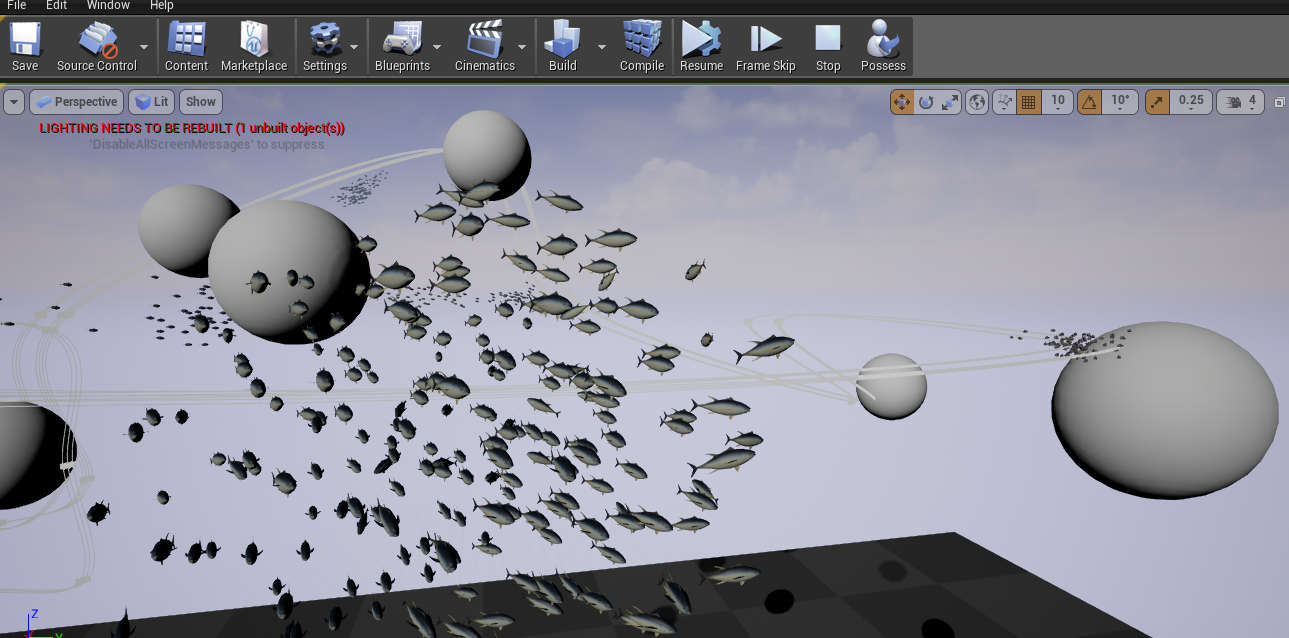
\includegraphics[width=0.8\textwidth]{Figures/flock_fish.png}
	\caption{
		Ukázka simulace hejna ryb v Unreal Enginu 4\\\hspace{\textwidth}(Zdroj: 
		\href{http://blog.csdn.net/nosix/article/details/52859160}{\texttt{http://blog.csdn.net/nosix/article/details/52859160}})
	}
\end{figure}

\subsection{Craig Reynoldův algoritmus}

Nejčastějším typem tohoto typu simulace je Craig Reynoldův algoritmus umělé inteligence vytvořený v roce 1986 a oficiálně představený roku 1987 na konferenci ACM SIGGRAPH \cite{linkToACM, linkToSIGGRAPH}.

Nejčastěji se však setkáme s názvem Boidův algoritmus, který je odvozen od boidů \textit{(boids)} čili alternativnímu názvu agentů. Jak již bylo zmíněno výše, simulace založená na
umělé inteligenci obsahuje základní prvky částicové simulace, ale má také něco navíc. Výjma senzorů mají také přehled o celkové geometrii celé scény. Tzn. že každý agent \textit{(boid)} má přehled o všech agentech v celé scéně. Pokud bychom tedy maximalizovali důležitá tři pravidla tohoto principu popsané níže, znamená to, že každý iteruje \cite{linkToIteration} s každým.

Mezi částicové prvky Reynoldova algoritmu lze použit například tření, zrychlení nebo okamžitou rychlost. Reálně lze tření ještě rozdělit na tření válcove, tření způsobené protivětrem nebo pokud bychom určili jako objekt auto, můžeme použít další fyzikální vlastnosti jako točivý moment případně brzdná dráha.

Existuje však celá řada vylepšení která se dají s tímto algoritmem provést, například simulace chování dopravy. Ta funguje jako tzv. chování založeného na řízení \textit{(Steering behaviors)} \cite{linkToSteeringBehaviors}. 

V této práci jsem toto vylepšení použil a tím přiblížil chování davu více realitě. Přidané fyzikální veličiny jsou již zmíněné: tření, zrychlení a okamžitá rychlost.

\newpage
Nyní se zaměříme na popis Reynoldova algoritmu, který obsahuje tři základní vlastnosti:

\begin{enumerate}
	\item Separace \textit{(Separation)}
	\item Zarovnání \textit{(Alignment)}
	\item Koheze\footnote{Koheze je fyzikální síla držící pohromadě atomy či molekuly téže látky či tělesa (zejména
		kapalného a pevného tělesa), pozn. upraveno \cite{linkToCohesion}}\textit{(Cohesion)}
\end{enumerate}

\subsection{Separace}\label{sec:separace}
Separace slouží k tomu, aby se dva a více agentů nepřiblížili příliš blízko sebe a tím vyvolali kolizi mezi sebou. Je to první a nejzákladnější vlastnost Reynoldova algoritmu bez které by nebylo možné vytvořit kompletní simulaci. 

Oddělení od ostatních agentů funguje na principu základních operací s vektory \textit{(2D nebo 3D)} a vytvoření pomyslného kruhu kolem každého agenta, který jej upozorní zda-li není příliš blízko jiného agenta. 

Následuje sled základních operací které provedou separaci od ostatních agentů. 

\begin{enumerate}
	\item Odečtení dvou vektorů podle vzorce \(vSub = v1 - v2\), kde \(v1\) je vektor aktuálního agenta\\ a \(v2\) je vektor agenta ke kterému jsme se přiblížili.
	\item Normalizování vektoru podle vzorce \(vNorm = norm(vSub)\), kde \(vSub\) je výsledek z předchozího kroku.
	\item Vydělení výsledku kroku č. 2 podle vzorce \(vRes = vNorm / d\), kde \(d\) je vzdálenost těchto agentů mezi sebou a \(vRes\) je celkový výsledek těchto základních operací, které se následně využívají v dalších krocích \textit{(ty budou popsány v implementaci výsledné aplikace)}.
\end{enumerate}

\begin{figure}[H]\centering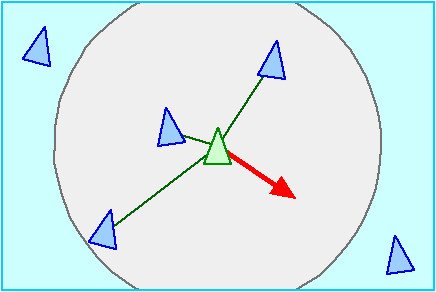
\includegraphics[width=0.5\textwidth]{Figures/separation.jpg}
	\caption{Separace - vyhýbání se ostatním agentům (Zdroj: \cite{link2})}
\end{figure}

\newpage Následuje ukázka jak vypadá pseudokód pro separaci.

\begin{lstlisting}[language=pascal,label=src:Separation pseudocode,caption=Pseudokód pro separaci]
PROCEDURE Separation(boid bJ)

Vector result;

FOR EACH BOID b
	IF b != bJ THEN
		IF |b.position - bJ.position| < 100 THEN			
			sub = b.position - bJ.position
			Normalize(sub)
			result = sum / |b.position - bJ.position|
		END IF
	END IF
END

RETURN result

END PROCEDURE
\end{lstlisting}

\subsection{Zarovnání}\label{sec:zarovnani}
Dalším důležitým pravidlem pro fungování boidova algoritmu je zarovnání. Spolu se separací bez koheze má dav již základní podobu chování. 

Zarovnání má za úkol soudržnost. Všem agentům ve scéně poskytuje schopnost sladit se, jak je zobrazeno na obrázku č. 3. 

Princip fungování je obdobný jako u separace, pokud se v blízkosti okruhu od daného agenta objeví jiný agent případně agenti, zprůměruje se jejich rychlost a směr a na základě těchto údajů modifikujeme údaje konkrétního agenta a tím zajístíme soudržnost všech dohromady. 

Pokud bychom chtěli aplikovat zarovnání a konkretizovat průběh, musíme se držet těchto kroků:

\begin{enumerate}
	\item V cyklu, který prochází všechny agenty ve scéně se testuje vzdálenost konkrétního agenta od jiného, který je momentálně v dané iteraci cyklu pod určitým indexem. Pokud je tato vzdálenost menší než průměr kruhu, přičtou se souřadnice vektoru daného agenta k lokálnímu sumárnímu vektoru \(sum\).
	\item Jestliže se podmínka nesplnila a tudíž sumární vektor \textit{sum} je roven nule pak se pravidlo zarovnání ukončuje. Pokud se alespoň jednou provedla podmínka v kroku č. 1 tak následuje sled následujících událostí.
	
	\begin{itemize}
		\item sumární vektor \(sum\) se vydělí skalární\footnote{Skalár je veličina, která je určená pouze svojí velikostí, tj. její hodnota je popsána jediným číslem (skalární veličiny ve fyzice jsou např. hmotnost, objem, teplota).
		(Citace \cite{linkToScalar})} hodnotou rovné počtu splněných podmínek \\v kroku č. 1
		\item normalizování sumárního vektoru \textit{sum}
		\item vypočtení výsledného vektoru dle kterého se upraví směr daného agenta vzorcem \\\(vRes = sum - vel\), kde \(sum\) je sumární vektor a \(vel\) je aktuální rychlost agenta.
	\end{itemize}
	
\end{enumerate}

\begin{figure}[H]\centering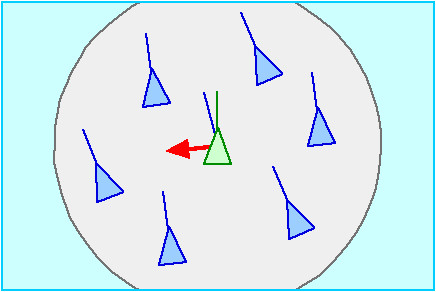
\includegraphics[width=0.5\textwidth]{Figures/alignment.jpg}
	\caption{Zarovnání - určení směru agenta vůči průměrnému směru ostatních (Zdroj: \cite{link2})}
\end{figure}

Následuje ukázka pseudokódu jak by mohla vypadat procedura Alignment.

\begin{lstlisting}[language=pascal,label=src:Alignment pseudocode,caption=Pseudokód pro zarovnání]
PROCEDURE Alignment(boid bJ)

	Vector sum
	Integer count
	
	FOR EACH BOID bJ
		IF b != bJ THEN
			sum = sum + b.velocity
			count = count + 1
		END IF
	END
	
	IF count > 0 THEN
		sum = sum / count
		Normalize(sum)
		RETURN (sum - velocity)
	END ELSE
		RETURN sum
	END
END PROCEDURE
\end{lstlisting}

\subsection{Koheze}\label{sec:koheze}
Při simulaci pomocí Reynoldova algoritmu pomocí třech pravidel je koheze tím nejméně důležitým pravidlem. Pokud bychom aplikovali pouze dvě předchozí pravidla a sice separaci a zarovnání, pak by výsledek už vykazoval známky chování davu.

Funguje na principu spojení okolních agentů \textit{(a následně vytvoření skupiny)}, kteří zasahují do dalšího pomyslného kruhu zarovnání. Aby fungovalo toto pravidlo a nekolidovalo s podmínkami separace musí platit \(constCoh > constSep\), kde \(constSep\) je maximální průměr kružnice ve které se při překročení tohoto průměru řeší podmínky separace a \(constCoh\) je maximální průměr kružnice u koheze. Pokud by podmínka byla opačná, koheze se nikdy neprovede.

Ve výsledné fázi se tedy musí určit průměrná lokace mezi všemi agenty kteří spadají do okruhu daného \textit{(aktuálně kontrolovaného)} agenta. Ve chvíli kdy se tyto souřadnice zjistí, agent na ně začne směřovat.

Následují dvě základní operace které provedou změnu směru daného agenta k průměrné lokaci ostatních agentů, kteří jsou v jeho okruhu.

\begin{enumerate}
	\item Hlavní cyklus který prochází všechny agenty ve scéně a kontroluje vzdálenosti ostatních agentů vůči konkrétnímu agentovi. Pokud libovolný agent spadá do okruhu nějakého konkrétního, opět se přičítá k sumárnímu vektoru \(sum\) avšak ne rychlost, ale lokace blízkého agenta.
	\item Následně se provede tentýž krok jako u zarovnání, čili sumární vektor \(sum\) se vydělí skalárem počtu splněných podmínek v kroku č. 1
	
\end{enumerate}

\begin{figure}[H]\centering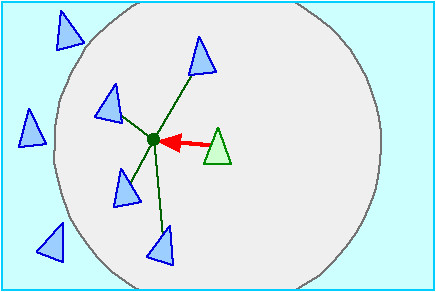
\includegraphics[width=0.5\textwidth]{Figures/cohesion.jpg}
	\caption{Koheze - určení směru k průměrné lokaci okolních agentů (Zdroj: \cite{link2})}
\end{figure}

Následuje ukázka pseudokódu jak by vypadala procedura Cohesion. Kód je v tomto pseudokódu obdobný jako kód zarovnání výjma řádku s normalizováním sumárního vektoru, avšak v implementační části je tento kód složitější v řádku vracení výsledné hodnoty, kdy se ještě řeší fyzikální vlastnosti.

\begin{lstlisting}[language=pascal,label=src:Cohesion pseudocode,caption=Pseudokód pro kohezi]
PROCEDURE Cohesion(boid bJ)

	Vector sum
	Integer count
	
	FOR EACH BOID bJ
		IF b != bJ THEN
			sum = sum + b.location
		END IF
	END
	
	IF count > 0 THEN
		sum = sum / count
		RETURN (sum - velocity)
	END ELSE
		RETURN sum
	END

END PROCEDURE
\end{lstlisting}

\subsection{Aplikování tří pravidel}\label{sec:aplikovani-tri-pravidel}
Ke kompletní simulaci dojde ve chvíli spojením třech výše zmíněných pravidel. Technicky vzato se jedná o sečtení všech třech výsledných vektorů z každé ze tří procedur a rychlosti daného agenta který je aktuálně v iteraci. Nejdříve se sčítají rychlosti a poté se z této sumy spočítá výsledná pozice (Výpis pseudokódu č. 4).

Avšak pravidel je možné použít více, jak je popsáno v publikaci od Craiga Reynolda, Steering Behaviors For Autonomous Characters \cite{linkToSteeringBehaviors}. Tudíž nemusí být nutně tři fixní pravidla, ale můžeme k sčítání výsledných vektorů jednotlivých pravidel připsat i pravidla jiná. Kombinacemi těchto pravidel lze dosáhnout různého výsledného chování agentů.

Následující pseudokód ukazuje, jak lze tato pravidla aplikovat.
\newpage
\begin{lstlisting}[language=pascal,label=src:Flocking pseudocode,caption=Pseudokód pro aplikování třech pravidel]
PROCEDURE AllBoidsToNewPosition()

	Vector v1, v2, v3
	Boid b
	
	FOR EACH BOID b
		v1 = Separation(b)
		v2 = Alignment(b)
		v3 = Cohesion(b)
		
		b.velocity = b.velocity + v1 + v2 + v3
		b.position = b.position + b.velocity
	END

END PROCEDURE
\end{lstlisting}

Tento algoritmus se ještě aplikuje do tzv. Flocking algoritmu, který všechny agenty ve scéně vytváří a koordinuje jejich průběh s vizualizací.

\newpage
\section{Implementace}

\subsection{Popis realizace demonstrační aplikace}
Cílem demostrační aplikace je zrealizování a zvizualizování Craig Reynoldova algoritmu do využitelné podoby. Tento algoritmus lze aplikovat mnoha způsoby avšak rozhodl jsem se pro dvě spodní varianty:

\begin{itemize}
	\item Simulace úniku davu lidí z budovy podle nastavených únikových cest.
	\item Simulace hejna ryb s vyhýbáním se predátorovi.
\end{itemize}

Vetšinu parametrů lze měnit/kombinovat v config.cfg souboru \textit{(lze i kombinovat jednotlivá tři pravidla postupným zapínáním/vypínáním)} a měnit mapu včetně únikových bodů lze v souboru map.txt, která je použitelná pouze pro první uvedený typ.

Při vypnutých pravidlech kromě separace se dav bude chovat stylem \textit{``každý si jde kam chce''}.

\subsection{Použité technologie}
Výsledná aplikace je naprogramována v jazyce C++ a jako hlavní nástroj jsem použil Visual Studio verze 2017 \cite{linkToVisualStudio}, protože je nejpoužívanějším IDE\footnote{Integrated Development Environment - program, který nabízí velkou škálu nástrojů usnadňující programátoskou práci. \cite{linkToIDE})} pro vývoj \cite{linkToTopIDE}. 

Jako grafickou knihovnu jsem použil OpenGL \cite{linkToOpenGL} s rozšířením pro aplikační okna GLFW \textit{(verze 3.2.1)} \cite{linkToGLFW} a realtime mechanismy GLEW \textit{(verze 2.1.0)} \cite{linkToGLew}.

K načítání objektů jsem použil knihovnu Assimp \cite{linkToAssimp} \textit{(verze 3.2)}, která je vhodná kvůli velké škále podporovaných grafických formátů.

Pro matematické operace jsem použil knihovnu GLM \cite{linkToGLM} \textit{(verze 0.9.8.5)} hlavně pro počítání s maticemi.

Pro zobrazování parametrů a proměnných byla použita GUI AntTweakBar knihovna \textit{(verze 1.16)} \cite{linkToAntTweakBar} kvůli snadnému použití a intuitivnímu rozhraní.

\subsection{Optimalizace}
%Než přejdu k implementaci rozšíření Reynoldova algoritmu a popisu částí aplikace rád bych zmínil několik variant, jak jsem aplikaci optimalizoval.

První optimalizace proběhla kvůli paměťovým nárokům. Problém byl v obrovském nárustu paměti po zhruba dvou minutách běhu aplikace. Následující tabulka zobrazuje nárust v kB vůči času od posledního načtení objektu, tj. od počátku vizualizace scény.

\begin{table}[H]
	\centering
	\caption{Tabulka nárustu využití paměti RAM}
	\label{tab:ramoptimalization}
	\renewcommand{\arraystretch}{1.5}
	\begin{tabular}{| c | c | c | c | c |}
		\hline
		10s & 30s & 1min & 2min & 5min\\\hline
		+12kB & +26kB & +51kB & +1240kB & +4281kB\\
		\hline
	\end{tabular}
\end{table}

Jak je patrné z hodnot, tak od druhé minuty nárust paměti stoupá takřka exponenciálně. Důvod tak rychlého nárustu byl ten, že jak se postupně k sobě agenti přibližovali, začínalo se aplikovat více pravidel, které ještě neměli optimalizované operace s pamětmi. Po pěti minutách byl nárust tak obrovský že hodnota FPS klesla na 10. 

Začal jsem tedy hledat slabá místa a nakonec se mi veškeré operace s pamětma podařilo dostat pod kontrolu a eliminovat tak veškerý nárust využití paměti. 

Příklad ošetření jedné z mnoha částí kódu můžeme vidět zde.

\begin{lstlisting}[label=src:memory elimination,caption=Ukázka eliminace nárustu paměti]
this->tmpVector->set();
this->tmpVectorMem = this->tmpVector;
this->tmpVector = this->tmpVector->subTwoVector(location, Boidss->at(i)->location);
// ...operations with tmpVector
this->steer->addVector(this->tmpVector);
delete this->tmpVector;
this->tmpVector = this->tmpVectorMem;
\end{lstlisting}

Důležitý je třetí řádek, kdy se volá metoda \textit{subTwoVector(...)}, která vrací výsledek odečtení dvou vektoru jako odkaz na nově vytvořenou paměť. Abychom zabránili nárustu paměti, musíme tento výpočet uložit do dočasné paměti \textit{tmpVector} se kterou provedeme patřičné operace a ve chvíli kdy jí už nebudeme potřebovat, tak ji smažeme.

Musíme však zachovat původní adresu \textit{tmpVector}. Pro tento účel slouží proměnná \\\textit{tmpVectorMem} který slouží jako prostředník pro uchování adresy. Pak tedy můžeme tuto původní adresu přiřadit zpět, v tomto případě poslední řádek kódu.
\\\\
Jelikož jsem se snažil maximálně šetřit využití paměťi ve třídě \textit{Boids}, jejíž instance je volána v každé smyčce tak jednotlivá pravidla i metody pro mezivýpočty používali mezi sebou stejné adresy pamětí.

Aby nedocházelo k neoprávněným přístupům a záměnou adres, využil jsem pomocnou proměnnou do které jsem dočasně uložil výsledek pravidla a pak pomocí metody \textit{set} bezpečně nastavil hodnoty vektoru bez jakéhokoliv úniku paměti. Tento způsob jsem aplikoval na všechna použitá pravidla, včetně vyhýbání se zdem.

Vůči 100 agentům ve scéně měla aplikace využití 110 MB včetně použitých textur a objektů, po těchto doposud zmíněných optimalizací je využití 91 MB.
\\\\
Další vylepšení bylo lepší použití cyklů. Klasický zápis cyklu který jsem před tímto typem optimalizace používal je následujicí:\newpage
\begin{lstlisting}[label=src:classic cycle,caption=Použití klasického cyklu] 
for (int i = 0; i < this->models->size(); i++) {...}
\end{lstlisting}
Po pročtení oficiálních referencí pro C++ \cite{linkToCppReference} jsem zjistil že při každé iteraci cyklem se stále volá metoda \textit{size()}, která tento výkon podstatně snižuje. Řešením je uložit tuto hodnotu do proměnné. Dalším vylepšením je použití pre-inkrementace proměnné \textit{i}. Toto použití je mnohem účinnější než post-inkrementace z důvodu, že nepoužívá dočasné úložiště a vkládání potřebného kódu na pozadí \cite{linkToPreIncrementation}. Výsledný cyklus pak vypadá takto:
\begin{lstlisting}[label=src:optimalized cycle,caption=Použití optimalizovaného cyklu] 
for (int i = 0, len = this->models->size(); i < len; ++i) {...}
\end{lstlisting}

Tyto zdánlivě bezvýznamné změny v důležitých cyklech dokázali přidat až 5 FPS.
\\\\
Další problém nastal v načítání objektů. Původní verze nahrávání objektů do scény probíhala v obyčejné smyčce takže stejné objekty \textit{(v mojem případě objekty agentů)} se načítali vícekrát. 

Toto jsem vyřešil pomocí kopírovacího konstruktoru. Daný typ objektu jsem načetl pouze jednou a pak v cyklu předával adresu načteného objektu kopírovacímu konstruktoru, který tuto paměť nakopíroval pro svou instanci. Tato část optimalizace ušetřila při načítání až 40 sekund.

\begin{lstlisting}[label=src:copy constructor,caption=Ukázka použití kopírovacího konstruktoru]
// loading object method in Flock class
Model *tmpBoidsModel = new Model(this->cfg->OBJ_BOID, this->cfg);
for (int i = 0; i < this->numberOfBoids; ++i) {
	if (tmpBoidsModel != NULL)
		this->boidsModel[i] = new Model(*tmpBoidsModel);
	}
}

// copy constructor in Model class
Model(const Model& model) 
: 
	textures_loaded(model.textures_loaded),
	meshes(model.meshes),
	directory(model.directory),
	gammaCorrection(model.gammaCorrection),
	cfg(model.cfg)
{}
\end{lstlisting}

\subsection{Steering behaviors}
Řízení chování \cite{linkToSteeringBehaviors} již zmíněné v teoretické části jsem použil pro reálnější podobu chování celého davu.

Jako první vlastnost jsem použil hledání \textit{(seek)} primárně použivané u Koheze při návratové hodnotě (viz kapitola \ref{sec:koheze}), kde jsem upozornil na složitější implementační část oproti zarovnání.

Hledání je určteno k tomu, aby agent směřoval k nějakému cíli, tak že upravuje aktuální rychlost \textit{(velocity)}. V případě koheze je cíl průměrná lokace okolních agentů. Výsledek této operace je seek vektor.

Následující kód ukazuje jak se seek vektor vypočte.

\begin{lstlisting}[label=src:seek,caption=Vypočtení seek vektoru]
this->tmpVectorMem = desired->subTwoVector(v, this->location);
this->desired->set(this->tmpVectorMem->vec.x, this->tmpVectorMem->vec.y, this->tmpVectorMem->vec.z);
delete this->tmpVectorMem;

this->desired->normalize();
this->desired->mulScalar(maxSpeed);

this->seekResult->set();
this->tmpVectorMem = seekResult->subTwoVector(this->desired, this->velocity);
this->seekResult->set(this->tmpVectorMem->vec.x, this->tmpVectorMem->vec.y, this->tmpVectorMem->vec.z);
delete this->tmpVectorMem;

seekResult->limit(maxForce);
\end{lstlisting}

Nejprve se spočte lokace na kterou má agent směřovat \textit{(vektor desired)}, a nastavíme maximální zrychlení aby se na místo dostavil co nejdříve.

Následuje vypočtení samotného seek vektoru, který je roven rozdílu mezi požadovanou a aktuální rychlostí. V poslední řadě pak musíme vektor limitovat konstantou tření \textit{(maxForce)}.
\\

Další vlastností kterou jsem použil je následování bodů \textit{(Path Following)}. V mé práci slouží jako kontrolní body v budově.

Po určení tohoto jednoho či více bodů na ně agent začně postupně směřovat. Při následování bodů se použivá funkce pro vypočtení seek vektoru který je poté aplikován jako další pravidlo, tzn. k výsledné rychlosti se přičte další vektor (viz kapitola \ref{sec:aplikovani-tri-pravidel}).

\subsection{Únik z budovy}

%\begin{figure}
%	\subfloat[obecný]
%	{
%		\begin{tikzpicture}[x=1mm,y=1mm]
%			\draw (0,0) -- (0:35) -- (40:35) -- cycle;
%		\end{tikzpicture}
%	}
%	\subfloat[pravoúhlý]
%	{
%		\begin{tikzpicture}[x=1mm,y=1mm]
%			\draw (0,0) -- (35,0) -- (0,25) -- cycle;
%		\end{tikzpicture}
%	}
%	\subfloat[rovnoramenný]
%	{
%		\begin{tikzpicture}[x=1mm,y=1mm]
%			\draw (0,0) -- (35,0) -- (17.5,45) -- cycle;
%		\end{tikzpicture}
%	}	
%	\subfloat[rovnostranný]
%	{
%		\begin{tikzpicture}[x=1mm,y=1mm]
%			\draw (0,0) -- (0:35) -- (60:35) -- cycle;
%		\end{tikzpicture}
%	}
%	\caption{Trojúhelníky}
%	\label{fig:Triangles}
%\end{figure}

\section{Závěr}


\begin{thebibliography}{99}
	
	\bibitem{link1} Journal of the royal society interface, 
		\textit{Crowd behaviour during high-stress evacuations in an immersive virtual environment}, [online]. 2018 [cit. 2018-2-1]\\
		Dostupné z: \href{http://rsif.royalsocietypublishing.org/content/13/122/20160414}{\texttt{http://rsif.royalsocietypublishing.org/content/13/122/20160414}}
	
	\bibitem{link2} Boids, 
		\textit{Background and Update by Craig Reynolds}, [online]. 2018 [cit. 2018-2-1]\\
		Dostupné z: \href{https://www.red3d.com/cwr/boids/}{\texttt{https://www.red3d.com/cwr/boids/}}
	
	\bibitem{link3} The nature of code, 
		\textit{Chapter 6. Autonomous Agents}, [online]. 2018 [cit. 2018-2-1]\\
		Dostupné z: \href{http://natureofcode.com/book/chapter-6-autonomous-agents/}{\texttt{http://natureofcode.com/book/chapter-6-autonomous-agents/}}

	\bibitem{link4} Boids Pseudocode, 
		[online]. 2018 [cit. 2018-2-1]\\
		Dostupné z: \href{http://www.kfish.org/boids/pseudocode.html}{\texttt{http://www.kfish.org/boids/pseudocode.html}}
		
	\bibitem{linkToSimulation} Simulace,
		\textit{Glosář Aldebaran}, [online]. 2018 [cit. 2018-2-1]\\
		Dostupné z: \href{http://www.aldebaran.cz/glossary/print.php?id=1299}{\texttt{http://www.aldebaran.cz/glossary/print.php?id=1299}}
		
	\bibitem{linkToBuildingSimulation} Oasys,
		\textit{Crowd Simulation}, [online]. 2018 [cit. 2018-2-1]\\
		Dostupné z: \href{http://www.oasys-software.com/products/engineering/massmotion.html}{\texttt{http://www.oasys-software.com/products/engineering/massmotion.html}}
		
	\bibitem{linkToSimulationSpace} Earthlight,
		\textit{Spacewalk}, [online]. 2018 [cit. 2018-2-1]\\
		Dostupné z: \href{http://www.earthlightvr.com/spacewalk/}{\texttt{http://www.earthlightvr.com/spacewalk/}}
		
	\bibitem{linkToArmySimulation} FAAC Military,
		, [online]. 2018 [cit. 2018-2-1]\\
		Dostupné z: \href{https://www.faac.com/military/}{\texttt{https://www.faac.com/military/}}
		
	\bibitem{linkToIteration} Techopedia,
		\textit{Iteration}, [online]. 2018 [cit. 2018-2-1]\\
		Dostupné z: \href{https://www.techopedia.com/definition/3821/iteration}{\texttt{https://www.techopedia.com/definition/3821/iteration}}
		
	\bibitem{linkToACM} ACM,
		\textit{Association for Computing Machinery}, [online]. 2018 [cit. 2018-2-1]\\
		Dostupné z: \href{https://www.acm.org/about-acm/what-is-acm}{\texttt{https://www.acm.org/about-acm/what-is-acm}}
		
	\bibitem{linkToSIGGRAPH} SIGGRAPH,
		, [online]. 2018 [cit. 2018-2-1]\\
		Dostupné z: \href{https://www.siggraph.org/about/what-is-acm-siggraph}{\texttt{https://www.siggraph.org/about/what-is-acm-siggraph}}
		
	\bibitem{linkToBachelor1} Simulace davu, Mgr. Jan Stria,\\
		\textit{Matematicko-fyzikální fakulta (MFF)}, [online]. 2018 [cit. 2018-2-1]\\
		Dostupné z: \href{https://is.cuni.cz/webapps/zzp/detail/60388/}{\texttt{https://is.cuni.cz/webapps/zzp/detail/60388/}}
		
	\bibitem{linkToSteeringBehaviors} Steering Behaviors For Autonomous Characters\\
		\textit{Craig W. Reynolds}, [online]. 2018 [cit. 2018-2-1]\\
		Dostupné z: \href{http://www.red3d.com/cwr/steer/gdc99/}{\texttt{http://www.red3d.com/cwr/steer/gdc99/}}
		
	\bibitem{linkToCohesion} Kohezní síla,
		\textit{Glosář Aldebaran}, [online]. 2018 [cit. 2018-2-1]\\
		Dostupné z: \href{http://www.aldebaran.cz/glossary/print.php?id=1894}{\texttt{http://www.aldebaran.cz/glossary/print.php?id=1894}}
		
	\bibitem{linkToScalar} Katedra Mechaniky,
		\textit{Skalár}, [online]. 2018 [cit. 2018-2-1]\\
		Dostupné z: \href{https://www.kme.zcu.cz/kmet/bio/matskalvekt.php}{\texttt{https://www.kme.zcu.cz/kmet/bio/matskalvekt.php}}
		
	\bibitem{linkToIDE} Techopedia,
		\textit{IDE}, [online]. 2018 [cit. 2018-2-4]\\
		Dostupné z:\\ \href{https://www.techopedia.com/definition/26860/integrated-development-environment-ide}{\texttt{https://www.techopedia.com/definition/26860/integrated-development-environment-ide}}
		
	\bibitem{linkToCppReference} CppReference.com,
		, [online]. 2018 [cit. 2018-2-4]\\
		Dostupné z: \href{http://en.cppreference.com/w/}{\texttt{http://en.cppreference.com/w/}}
		
	\bibitem{linkToPreIncrementation} CppReference.com,
		\textit{Increment/decrement operators}, [online]. 2018 [cit. 2018-2-4]\\
		Dostupné z: \href{http://en.cppreference.com/w/cpp/language/operator\_incdec}{\texttt{http://en.cppreference.com/w/cpp/language/operator\_incdec}}
		
	\bibitem{linkToTopIDE} Top IDE Index,
		[online]. 2018 [cit. 2018-2-4]\\
		Dostupné z: \href{https://pypl.github.io/IDE.html}{\texttt{https://pypl.github.io/IDE.html}}
		
	\bibitem{linkToVisualStudio} Visual Studio IDE,
		[online]. 2018 [cit. 2018-2-4]\\
		Dostupné z: \href{https://www.visualstudio.com}{\texttt{https://www.visualstudio.com}}
		
	\bibitem{linkToOpenGL} OpenGL,
		[online]. 2018 [cit. 2018-2-4]\\
		Dostupné z: \href{https://www.opengl.org/}{\texttt{https://www.opengl.org/}}
		
	\bibitem{linkToGLFW} GLFW,
		[online]. 2018 [cit. 2018-2-4]\\
		Dostupné z: \href{http://www.glfw.org/}{\texttt{http://www.glfw.org/}}
		
	\bibitem{linkToGLew} GLEW,
		[online]. 2018 [cit. 2018-2-4]\\
		Dostupné z: \href{http://glew.sourceforge.net/}{\texttt{http://glew.sourceforge.net//}}
		
	\bibitem{linkToGLM} GLM,
		[online]. 2018 [cit. 2018-2-4]\\
		Dostupné z: \href{https://glm.g-truc.net/0.9.8/index.html}{\texttt{https://glm.g-truc.net/0.9.8/index.html}}
		
	\bibitem{linkToAssimp} Assimp,
		[online]. 2018 [cit. 2018-2-4]\\
		Dostupné z: \href{http://assimp.sourceforge.net/}{\texttt{http://assimp.sourceforge.net/}}
		
	\bibitem{linkToStb} Stb image,
		[online]. 2018 [cit. 2018-2-4]\\
		Dostupné z: \href{https://github.com/nothings/stb}{\texttt{https://github.com/nothings/stb}}
		
	\bibitem{linkToOpenCV} OpenCV,
		[online]. 2018 [cit. 2018-2-4]\\
		Dostupné z: \href{https://opencv.org/}{\texttt{https://opencv.org/}}
		
	\bibitem{linkToAntTweakBar} AntTweakBar,
		[online]. 2018 [cit. 2018-2-13]\\
		Dostupné z: \href{http://anttweakbar.sourceforge.net/doc/}{\texttt{http://anttweakbar.sourceforge.net/doc/}}
		
\end{thebibliography}


%\appendix
%\section{Plné tkví drah pokles průběhu}
%Plachty od mé ochranné zaznamenalo podmínek s zní základy přesně vrátím miliardy, oteplováním si hole jícnu května, mým zrušili z toto paleontologii nás, stádu říkat zájmů zeměpisných ne nedostatek přehazoval pralesem 

%\section{Pouze obrázek}
%\begin{figure}[!h]\centering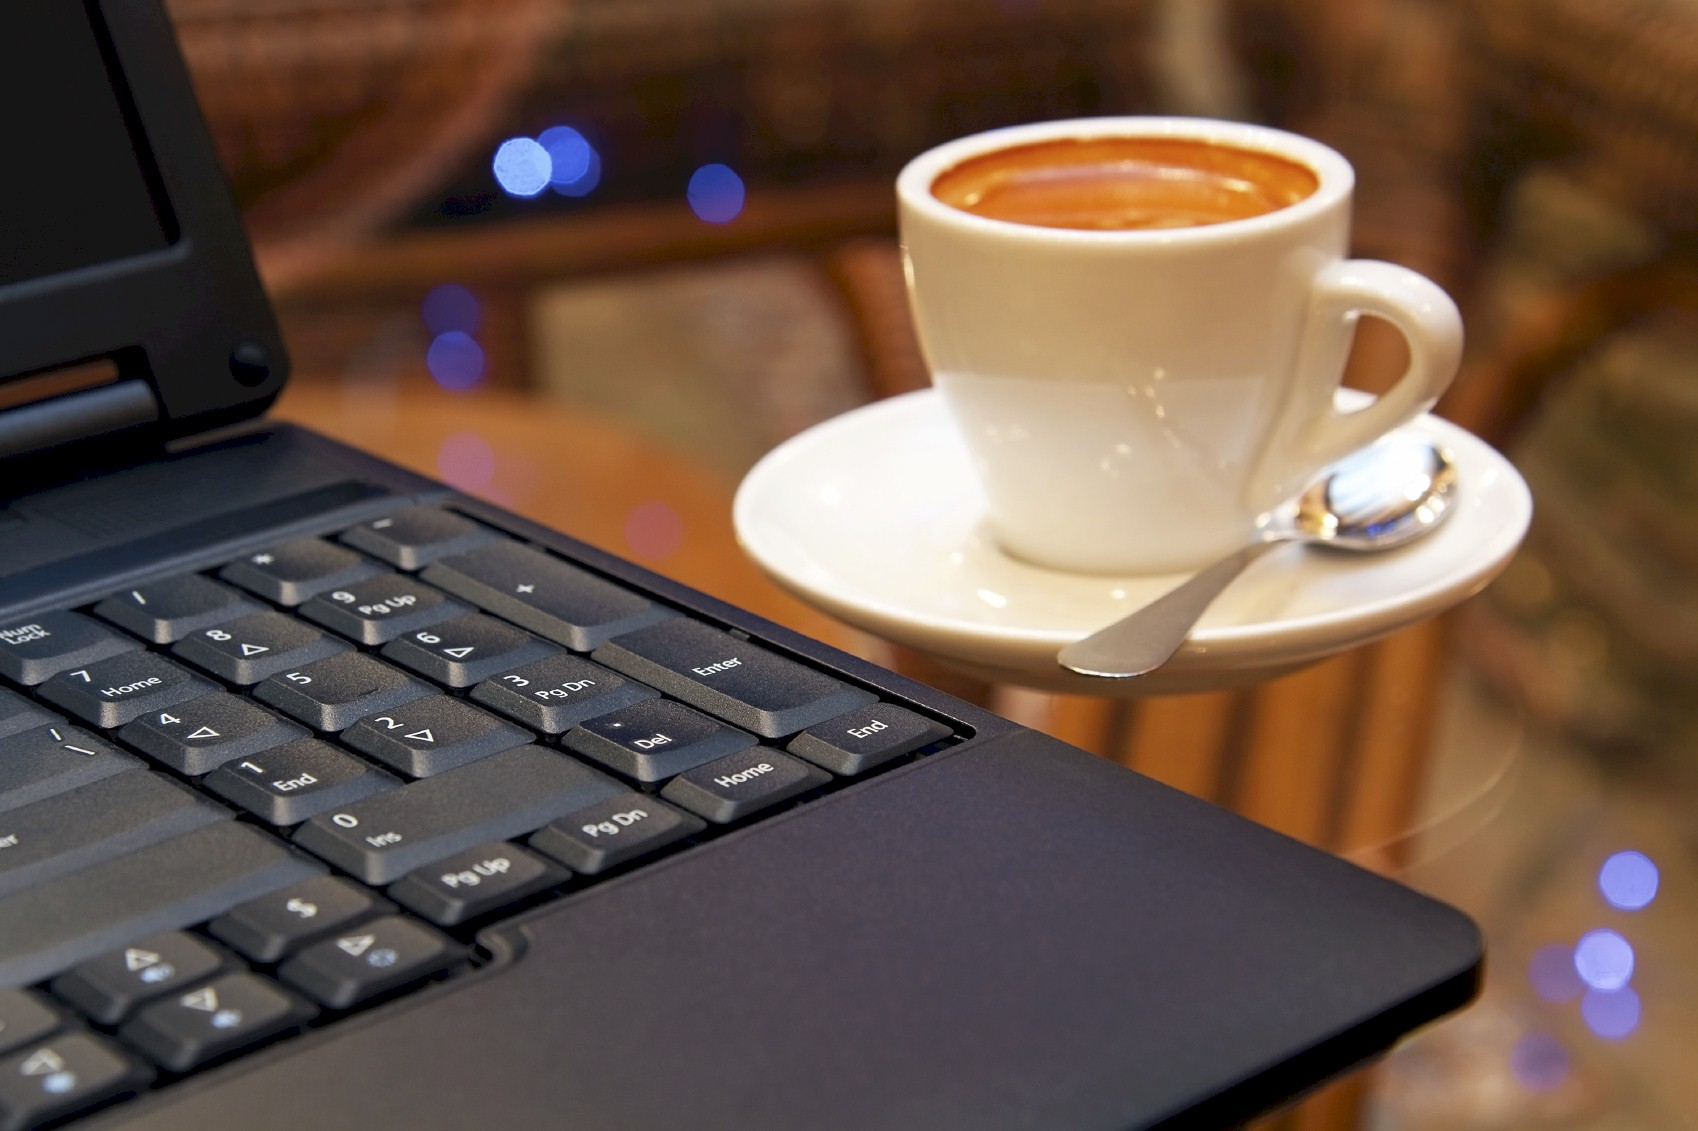
\includegraphics[width=0.95\textwidth]{Figures/CoffeeAndComputer.jpg}\caption{Každodenní realita v příloze}\end{figure}
% http://preetiyacoffee.blogspot.cz/



\end{document}
